\documentclass[master=elt,masteroption=eo,oneside]{kulemt}
%\pagestyle{}
\usepackage{titlesec}

\setup{title={Ontwerp van een quadcoptersturing in VHDL },
  author={Andries Gert-Jan},
  promotor={Ing.\ Sammy~Verslype},
  assessor = {Ing.\ Sammy~Verslype},
  assistant={Ing.\ Sammy~Verslype}}

% De volgende \setup mag verwijderd worden als geen fiche gewenst is.
%\setup{filingcard,
%    translatedtitle={place english translation of title here}, 
%    udc=621.3,
%    shortabstract={Hier komt een heel bondig abstract van hooguit 500
%    woorden. \LaTeX\ commando's mogen hier gebruikt worden. Blanco lijnen
%    (of het commando \texttt{\string\pa r}) zijn wel niet toegelaten!
%    \endgraf \lipsum[2]}}

\usepackage{graphicx}
\usepackage{titlesec}
\usepackage{listings}
\usepackage{color}
\usepackage{float}
\usepackage{amsmath}
\usepackage{booktabs}
\usepackage{upquote}
\usepackage{gensymb}
\usepackage{eurosym}
\usepackage{array}
\usepackage{bytefield}
\usepackage{siunitx}
\usepackage{xcolor}
%\usepackage[usenames,dvipsnames]{xcolor}
\usepackage{booktabs,colortbl, array}
\usepackage{pgfplotstable}
\usepackage{csquotes}
\usepackage{environ}
\usepackage[bottom]{footmisc}
\usepackage{pdfpages}
\usepackage{array,tabularx}
\usepackage{caption}
\usepackage{subcaption}
\usepackage{tikz}
\usepackage[export]{adjustbox}
\usepackage{float}

\lstdefinelanguage{VHDL}{
  morekeywords=[1]{
    library,use,all,entity,is,port,in,out,end,architecture,of,
    begin,and,or,Not,downto,ALL
  },
  morekeywords=[2]{
    STD_LOGIC_VECTOR,STD_LOGIC,IEEE,STD_LOGIC_1164,
    NUMERIC_STD,STD_LOGIC_ARITH,STD_LOGIC_UNSIGNED,std_logic_vector,
    std_logic
  },
  morecomment=[l]--
}

\colorlet{keyword}{blue!100!black!80}
\colorlet{STD}{violet}
\colorlet{comment}{blue}
\lstdefinestyle{vhdl}{
  language     = VHDL,
  basicstyle   = \footnotesize \ttfamily,
  keywordstyle = [1]\color{keyword}\bfseries,
  keywordstyle = [2]\color{STD}\bfseries,
  commentstyle = \color{comment}
  breaklines=true,                % sets automatic line breaking
  tabsize=3                                % sets default tabsize to 2 spaces
}


\newenvironment{conditions*}
  {\par\vspace{\abovedisplayskip}\noindent
   \tabularx{\columnwidth}{>{$}l<{$} @{\ : } >{\raggedright\arraybackslash}X}}
  {\endtabularx\par\vspace{\belowdisplayskip}}

%%%%%%%%%%%%%%%%%%%%%%%%%%%%%%%%%%%%%%%%%%%%%%%%%%%%%%%%%%%%%%%%%%%%%%%%%%%%%%%
\makeatletter
\newsavebox{\measure@tikzpicture}
\NewEnviron{scaletikzpicturetowidth}[1]{%
  \def\tikz@width{#1}%
  \def\tikzscale{1}\begin{lrbox}{\measure@tikzpicture}%
  \BODY
  \end{lrbox}%
  \pgfmathparse{#1/\wd\measure@tikzpicture}%
  \edef\tikzscale{\pgfmathresult}%
  \BODY
}
\makeatother

\newcommand{\getsizes}[2]% width, height
{   \path (current bounding box.south west);
    \pgfgetlastxy{\xsw}{\ysw}
    \path (current bounding box.north east);
    \pgfgetlastxy{\xne}{\yne}
    \pgfmathsetmacro{\picwidth}{(\xne-\xsw)/28.453}
    \pgfmathsetmacro{\picheight}{(\yne-\ysw)/28.453}
    \pgfmathsetmacro{\picxscale}{#1/\picwidth}
    \pgfmathsetmacro{\picyscale}{#2/\picheight}
    \xdef\xsca{\picxscale}
    \xdef\ysca{\picyscale}
}

\newcommand{\xyscaledtikz}[3]% draw commands, width, height
{ \smash{\vphantom{
    \begin{tikzpicture}
        #1
        \getsizes{#2}{#3}
    \end{tikzpicture}
    }}
    \begin{tikzpicture}[xscale=\xsca,yscale=\ysca]
        #1
    \end{tikzpicture}
}

\pgfplotsset{compat=1.8}

%%listings
\definecolor{mygreen}{rgb}{0,0.6,0}
\definecolor{mygray}{rgb}{0.5,0.5,0.5}
\definecolor{mymauve}{rgb}{0.58,0,0.82}
\definecolor{lightgray}{rgb}{.9,.9,.9}
%%tables
\definecolor{rulecolor}{RGB}{0,0,0}
\definecolor{tableheadcolor}{gray}{0.92}

%%commands
\newcommand{\topline}{ 
        \arrayrulecolor{rulecolor}\specialrule{0.1em}{\abovetopsep}{0pt}
        \arrayrulecolor{tableheadcolor}\specialrule{\belowrulesep}{0pt}{0pt}
        \arrayrulecolor{rulecolor}}

\newcommand{\midtopline}{ 
        \arrayrulecolor{tableheadcolor}\specialrule{\aboverulesep}{0pt}{0pt}
        \arrayrulecolor{rulecolor}\specialrule{\lightrulewidth}{0pt}{0pt}
        \arrayrulecolor{white}\specialrule{\belowrulesep}{0pt}{0pt}
        \arrayrulecolor{rulecolor}}

\newcommand{\bottomline}{ 
        \arrayrulecolor{white}\specialrule{\aboverulesep}{0pt}{0pt}
        \arrayrulecolor{rulecolor} 
        \specialrule{\heavyrulewidth}{0pt}{\belowbottomsep}}

\newcommand{\midheader}[2]{
        \midrule\topmidheader{#1}{#2}}

\newcommand\topmidheader[2]{\multicolumn{#1}{c}{\textsc{#2}}\\
                \addlinespace[0.5ex]}

\newcolumntype{C}{>{\raggedright\arraybackslash}p{7cm}}
\newcolumntype{D}{>{\raggedright\arraybackslash}p{3cm}}
\newcolumntype{A}{>{\raggedright\arraybackslash}p{2cm}}
\newcolumntype{B}{>{\raggedright\arraybackslash}p{4cm}}
\newcolumntype{F}{>{\raggedright\arraybackslash}p{0.20\textwidth}}
\newcolumntype{G}{>{\raggedright\arraybackslash}p{0.15\textwidth}}
\newcolumntype{I}{>{\raggedright\arraybackslash}p{0.25\textwidth}}
\newcolumntype{J}{>{\raggedright\arraybackslash}p{0.35\textwidth}}
\newcolumntype{K}{>{\raggedright\arraybackslash}p{0.45\textwidth}}

%%Tables
\pgfplotstableset{
        normal/.style ={
        header=true,
        string type,
        %font=\addfontfeature{Numbers={Monospaced}}\small,
        column type=l,
        every odd row/.style={
            before row=
        },
        every head row/.style={
            before row={\topline\rowcolor{tableheadcolor}},
            after row={\midtopline}
        },
        every last row/.style={
            after row=\bottomline
        },
        col sep=&,
        row sep=\\
    },
    center/.style ={
        header=true,
        string type,
        %font=\addfontfeature{Numbers={Monospaced}}\small,
        column type=c,
        every odd row/.style={
            before row=
        },
        every head row/.style={
            before row={\topline\rowcolor{tableheadcolor}},
            after row={\midtopline}
        },
        every last row/.style={
            after row=\bottomline
        },
        col sep=&,
        row sep=\\
    }
}


% monospaced font with bold variant




%%%%%%%%%%%%%%%%%%%%%%%%%%%%%%%%%%%%%%%%%%%%%%%%%%%%%%%%%%%%%%%%%%%%%%%%%%%%%%%


% Kies de fonts voor de gewone tekst, bv. Latin Modern
%\setup{font=lm} %T en nog een aantal andere letters zijn kleiner dan andere, dit trekt echt op niets in bvb 'NTC'. Zonder die instelling is er eensgezindheid onder de hoofdletters
\setlength{\parskip}{1em}
\setlength\parindent{0pt}

\titleformat{\chapter}[display]
    {\normalfont\huge\bfseries}{\chaptertitlename\ \thechapter}{20pt}{\Huge}
\titlespacing*{\chapter}{0pt}{-40pt}{10pt}



%%%%%%%
% Om wat tekst te genereren wordt hier het lipsum pakket gebruikt.
% Bij een echte masterproef heb je dit natuurlijk nooit nodig!
\IfFileExists{lipsum.sty}%
 {\usepackage{lipsum}\setlipsumdefault{11-13}}%
 {\newcommand{\lipsum}[1][11-13]{\par Hier komt wat tekst: lipsum ##1.\par}}
%%%%%%%


\begin{document}

%----------------------------------------------------------------------------------------------------------------------------------------------------
%\begin{preface}
%  \par Het tot stand komen van deze masterproef is het resultaat van een samenwerking tussen heel wat mensen. Van deze gelegenheid wensen wij gebruik te maken om alle personen te bedanken die rechtstreeks en onrechtstreeks bijgedragen hebben aan het tot stand komen van deze masterproef. 
%  \par Eerst en vooral willen wij alle docenten bedanken,  betrokken bij onze opleiding, meerbepaald de docenten van de afdeling electronica-ICT. In het bijzonder willen wij ook onze buitenpromotor, Crombez Pieter, bedanken voor de uitstekende begeleiding  van onze masterproef. Verder bedanken wij ook onze binnenpromotor Verslype Sammy en opleidingshoofd Peuteman Joan. Tot slot bedanken wij ook onze ouders en familie om ons de kans te geven deze opleiding te volgen. 
%\end{preface}
%----------------------------------------------------------------------------------------------------------------------------------------------------

\tableofcontents*

%-------------------------
\begin{abstract}
    \par In dit projectlab wordt een quadcoptersturing ontworpen op een FGPA. Aan de hand van een PID regeling wordt de stabilisatie voorzien rond de drie bewegingsassen van de quadcopter. Vanwege de beperkte hoeveelheid resources die op de FPGA aanwezig zijn, dient er in het hardware ontwerp rekening gehouden te worden met deze beperking. Verschillende iteraties en methodieken worden ondernomen om de benodigde resources voor deze PID regeling tot een minima te beperken. Zo werd onderzocht of er gebruik gemaakt kan worden van de snelle DSP48 slices. Daarnaast wordt ook een implementatie gemaakt aan de hand van de IP CoreGenerator multiplier. 

    \par Naast het ontwerpen van een PID controller worden ook verschillende andere systeemcomponenten ontworpen. Een PWM generator zal de BLDC motoren voorzien van een gepast PWM signaal dat voldoet aan de frequentievoorschriften van de motorfabrikant. Om het juiste signaal voor elke motor te genereren, wordt een motormixing unit ontworpen die het motormixingalgoritme implementeert. 

    \par Communicatie met de buitenwereld wordt voorzien door middel van een SPI slave interface. Deze interface wordt gebruikt om sensorwaarden te ontvangen, maar laat de gebruiker ook toe bepaalde registers uit te lezen of in te stellen.

    \par Alle hardware wordt gesimuleerd en vervolgens getest op een FPGA. Via Matlab en Simulink worden vooraf de nodige berekeningen en simulaties uitgevoerd die als basis voor het FPGA design dienen.

    \par Naast de hardware wordt ook het quadcopterframe volledig ontworpen. Dit frame wordt zodanig ontworpen dat het uit verschillende onderdelen bestaat die door een 3D printer vervaardigd kunnen worden.
\end{abstract}
%-------------------------

%include the symbols and abbreviations list from different file to keep it all organized
% Een lijst van figuren en tabellen is optioneel
%\listoffigures
%\listoftables
% Bij een beperkt aantal figuren en tabellen gebruik je liever het volgende:
\listoffiguresandtables
% De lijst van symbolen is eveneens optioneel.
% Deze lijst moet wel manueel aangemaakt worden, bv. als volgt:
\chapter{Lijst van afkortingen}

\begin{flushleft}
  \renewcommand{\arraystretch}{1.1}
  \begin{tabularx}{\textwidth}{@{}p{12mm}X@{}}
			ADC 					& Analog to Digital Converter\\
			ARM 					& Advanced RISC Machines\\			
			AHRS					& Attitude and Heading Reference System\\
			BLDC					& Brushless DC\\
			CPHA					& Phase Polarity\\
			CPOL					& Clock Polarity\\
			DC						& Direct Current \\
			DMP						& Digital Motion Processing\\
			DSP 					& Digital Signal Processing\\		
			ESC						& Engine Speed Controller\\
			FPGA					& Field Programmable Gate Array 	\\
			I\textsuperscript{2}C 	& Inter-IC bus\\		
			IC 						& Integrated circuit\\		
			IMU						& Inertial Measurement Unit\\
			IO						& Input Output\\
			IP						& Intellectual Property\\
			KU 						& Katholieke Universiteit\\		
			KUL 					& Katholieke Universiteit Leuven\\		
			MAC 					& Multiply and Accumulate\\		
			MAVLink					& Micro Air Vehicle Communication Protocol	\\
			MHz 					& Megahertz\\		
			MISO					& Master In Slave Out\\
			MOSI					& Master Out Slave In\\
			PCB 					& Printed Circuit Board\\		
			PID						& Proportioneel Integrerend Differenti\"erend	\\
			PWM						& Pulse Width Modulation\\
			RF						& Radio Frequency\\
			SCLK					& Serial Clock Line\\
			SM						& Sliding Mode	\\
			SPI 					& Serial Peripheral Interface\\		
			SS 						& Slave Select\\
			UART 					& Universal Asynchronous Receiver Transmitter\\		
			USB						& Universal Serial Bus\\		
			VHDL					& Very High Speed Integrated Circuit Hardware Description Language\\




  \end{tabularx}
\end{flushleft}

% Nu begint de eigenlijke tekst
\mainmatter

\chapter{Inleiding}
	
	\par In dit verslag worden de resultaten van het projectlab toegelicht. Elke stap die werd genomen om het eindresultaat te bekomen wordt kort besproken, alsook de moeilijkheden die zich hebben voorgedaan tijdens de ontwikkeling. Tenslotte wordt ook een besluit gevormd over het gehele project en worden de toekomstmogelijkheden kort toegelicht. 

	\section{Omschrijving van de opdracht}

		\par Het project is onderverdeeld in twee grote onderdelen. Enerzijds is er het stabilisatiealgoritme voor de quadcopter en anderzijds is er de sturing, hardware design en optical flowintegratie. De focus van het project zal gelegd worden op de stabiliteitsnelheid van het eindresultaat. Het onderdeel met het stabilisatie-algoritme omvat het genereren van PWM signalen die de motoren aansturen. Hiervoor is sensordata nodig van bijvoorbeeld een gyroscoop, accelerometer, magnetometer en barometer. Om de ruis uit deze metingen weg te filteren zal gebruik gemaakt worden van een filter, bijvoorbeeld Kalman, die ook in de FPGA zal ge\"integreerd worden. Naast data van sensoren zal de FPGA ook informatie ontvangen van een extra processor. Op deze extra processor wordt de communicatie met de grond voorzien (besturing), alsook een optical flow algoritme. 

		\par De stabilisatie zelf zal uitgevoerd worden door een PID of SM (sliding mode) dat ook op de FPGA zal ge\"integreerd worden. De instellingen van het stabilisatie-algoritme zullen gemaakt worden door middel van registers die door de externe processor kunnen ingesteld worden via I\textsuperscript{2}C of SPI. Via deze registers kan ook de actuele sensor- en systeeminformatie opgevraagd worden. De hardware bestaat uit een zelf te ontwikkelen printplaat gebaseerd op een FPGA (Spartan 6) die de stabilisatie en verwerking van de inputs verzorgt. Daarnaast bevat het ook een microcontroller die de communicatie voorziet, alsook de beeldverwerking voor de optical flow en het batterijbeheer. De communicatie zou verlopen volgens het MAVLink protocol, een gestandaardiseerd protocol dat communicatie voorziet onafhankelijk van de fysische laag waarop dit gebeurt. Een keuze voor het beste kanaal maakt ook deel uit van dit project. 
\newpage
		\par Optical flow detectie voorziet de  mogelijkheid om de horizontale ongewenste bewegingen tegen te werken en dus de quadcopter op een vaste positie te houden. De sturing voor de BLDC motoren wordt zelf ge\"implementeerd en vindt plaats op externe processoren die elk instaan voor \'e\'en enkele motor. Het FPGA ontwikkelbord waarmee gewerkt zal worden is het Mojo bord met een Spartan 6 processor. Dit bord zal zelf aangekocht worden. Verder zal ook een MPU9250 gebruikt worden om accelero-, magneto- en gyro-data te verzamelen. De andere sensoren die gebruikt zullen worden dienen te worden bepaald tijdens de looptijd van het project. 

		\par Wanneer alle sensoren getest zijn, worden ze samen met de FPGA (niet het ontwikkelbord) op de zelf ontworpen printplaat geplaatst om zo een quadcoptersturing te verkrijgen die onafhankelijk is van een ontwikkelbord of opgelegde pinout. Deze wordt gemonteerd op de quadcopter structuur die gemaakt zal worden door middel van een 3D printer. Dit maakt het nadien ook mogelijk om bij een crash een bepaald onderdeel snel te reproduceren.

		\par Dit projectlab kan worden opgesplitst in verschillende milestones.
			
		\begin{itemize}
			\item  Stabilisatie en sturing (Gert-Jan)
				\begin{itemize}
					\item Uitlezen sensoren
					\item Uitfilteren van ruis op sensordata
					\item Stabilisatie-algoritme PID/SM
					\item Instellingsmogelijkheid van registers
					\item Ontwerp van quadcopterframe
				\end{itemize}
			\item  Hardware en optical flow (Nick)
				\begin{itemize}
					\item Ontwerpen printplaat
					\item Implementeren MAVLink
					\item Selecteren communicatiekanaal
					\item Optical flow
					\item BLDC motor sturing
					\item Return to home functie
				\end{itemize}
		\end{itemize}
\newpage
	\section{Planning en werkwijze}

		\par De algemene werkwijze van het project kan onderverdeeld worden in vier grote blokken.

			\begin{description}
				
				\item[Onderzoek:] In deze fase van het project wordt een onderzoek uitgevoerd met betrekking tot quadcopters. Er wordt gekeken naar hoe een quadcopter bestuurd wordt en via welke algoritmen dit kan gebeuren. Daarnaast zal ook een studie gemaakt worden naar het implementeren van een PID-controller in een FPGA. Via simulaties in het programma simulink kunnen de algoritmen ge\"evalueerd worden.

				\item[Implementatie:] In deze fase worden de onderzoeksresultaten omgezet in code. Via het programma Xilinx ISE en Vivado wordt de implementatie voorzien op een FPGA. Aan de hand van het programma Modelsim worden de hardwaredesigns ge\"evalueerd alvorens deze op de FPGA worden getest.

				\item[Testen:] Wanneer de hardware gevalideerd is door middel van een testbench, kan deze getest worden op de FPGA zelf. Blok per blok zullen de nodige testen uitgevoerd worden en bijgestuurd waar nodig. 

				\item[Reflectie:] Elk ontworpen blok zal onderworpen worden aan een kritische evaluatie. Hierbij wordt gekeken naar performantie, accuraatheid en werking binnen het geheel. Waar nodig wordt bijgestuurd. Regelmatige communicatie met medestudent Nick, die de hardware (PCB) ontwerpt is hierbij nodig.

			\end{description}

		\par Een beknopte projectplanning wordt hieronder weergegeven. Een uitgebreide versie hiervan is terug te vinden in appendix \ref{app:A} op pagina \pageref{app:A}. Deze uitgebreide versie houdt rekening met de initi\"ele planning. Hieronder is het werkelijke verloop van het project weergegeven.

			\begin{itemize}
				
				\item[Week 1:] 
					\begin{itemize}
						\item Keuze maken van het project uit de aangeboden projecten.  
						\item Registreren van het gekozen project.
					\end{itemize}

				\item[Week 2:] 
					\begin{itemize}
						\item Indienen van de projectplanning.
						\item Onderzoek naar quadcopters en besturing.
						\item Studie PID en digitalisering.
						\item Studie IMU sensoren.
					\end{itemize}

				\item[Week 3:]
					\begin{itemize}
						\item Simulatie van PID algoritme in Matlab en Simulink.
						\item Theoretisch ontwerp van PID door middel van DSP48 slices.
						\item Kennismaking Mojo ontwikelbord en Xilinx ISE.
					\end{itemize}				

				\item[Week 4:]
					\begin{itemize}
						\item Tussentijdse presentatie van het project.
						\item Implementatie van PID door middel van DSP48 slices .
						\item Evaluatie van PID implementatie en bijsturing.
						\item Ontwerp van quadcopter frame in Inventor.
					\end{itemize}					

				\item[Week 5:]
					\begin{itemize}
						\item Ontwerp SPI slave interface in VHDL.
						\item Bijsturen PID ontwerp, implementatie met behulp van IP core multiplier.
						\item Validatie van ontwerp door middel van testbenches.

					\end{itemize}					

				\item[Week 6:]
					\begin{itemize}
						\item Bijsturen PID ontwerp, implementatie met behulp van IP core multiplier.
						\item Validatie van ontwerp door middel van testbenches.
						\item Ontwerp SPI slave interface aanpassen aan Mojo SPI.
						\item Testprint van quadcopter arm en stevigheidstest.
					\end{itemize}					

				\item[Week 7:]
					\begin{itemize}
						\item Bijsturen ontwerp van quadcopter arm.
						\item Printen van vier quadcopterarmen.
						\item Ontwerp van PWM generator in VHDL.
					\end{itemize}					

				\item[Week 8:]
					\begin{itemize}
						\item Tussentijdse presentatie van het project.
						\item Testen PWM generator op Mojo. 
						\item Testen van SPI slave interface op Mojo. 
						\item Ontwerp bijsturen waar nodig.
					\end{itemize}					

				\item[Week 9:]
					\begin{itemize}
						\item PID regeling aanpassen naar multiplexing om resources te besparen op de FPGA.
						\item Valideren van het nieuwe PID ontwerp.
						\item Testen van PWM en SPI samen op Mojo bord.
					\end{itemize}					

				\item[Week 10:]
					\begin{itemize}
						\item Ontwerpen van motormixingalgoritme in VHDL.
						\item Optimalisatie van PID controller.
						\item Implementatie van registers.
					\end{itemize}					

				\item[Week 11:]
					\begin{itemize}
						\item Labobad Gent.
					\end{itemize}					

				\item[Week 12:]
					\begin{itemize}
						\item Eindpresentatie en demo van het labproject.
					\end{itemize}								

				\item[Week 14:]
					\begin{itemize}
						\item Indienen van het eindverslag.
					\end{itemize}

			\end{itemize}
\chapter{Vooronderzoek}

	\par In dit hoofdstuk zullen de verschillende resultaten van het vooronderzoek besproken worden. Ook de simulaties in het programma simulink worden kort toegelicht. Op het einde van dit hoofdstuk wordt een compleet systeemoverzicht weergegeven. 

	\section{Quadcopters}

		\subsection{Wat is een quadcopter}
			
			\par Een quadcopter, ook wel quadrocopter genoemd, is een hefschroefvliegtuig dat, zoals de naam al doet vermoeden, aangedreven wordt door vier motoren. In tegenstelling tot een conventionele helikopter maakt een quadcopter gebruik van symmetrisch hellende propellors die in groepen van twee dezelfde draairichting hebben. Op deze manier wordt de tolbeweging die ontstaat door de krachtwerking van de motoren tegengewerkt en gereduceerd tot nul. Dit zorgt ervoor dat de quadcopter tijdens de vlucht niet rondtolt. Bij een klassieke helikopter wordt het opheffen van deze kracht voorzien door de staartrotor.

				\begin{figure}[H]					  
					  \centering
					  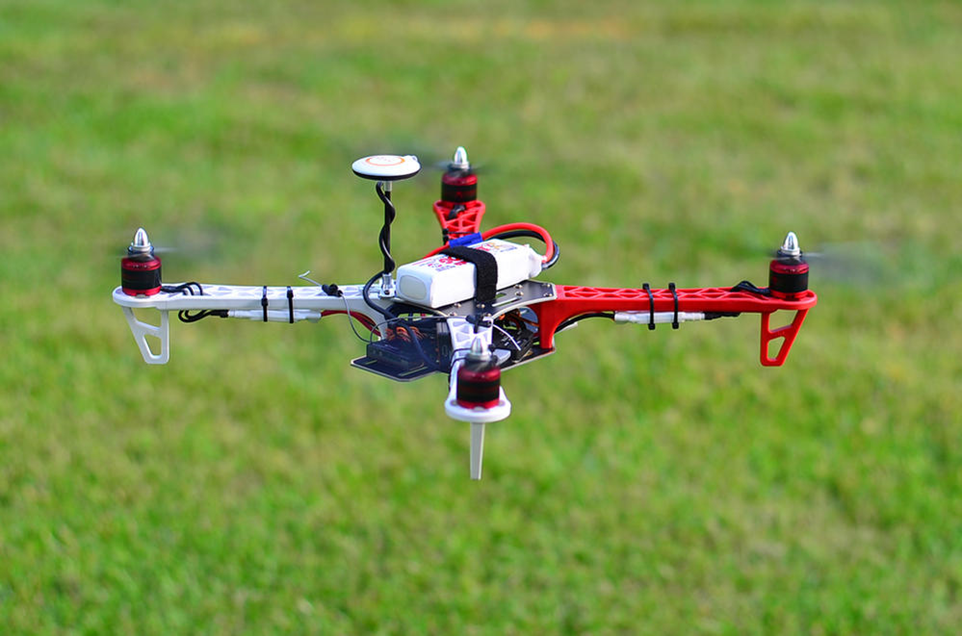
\includegraphics[width=0.5\textwidth]{Vooronderzoek/quad_foto.png}
					  \caption{Quadcopter in actie}
					  \label{quadcopter_foto}
				\end{figure}

			\par Een quadcopter is opgebouwd uit een frame dat vier armen bevat. Op het uiteinde van deze armen zijn de motoren (brushless DC) bevestigd. Om de motoren aan te sturen wordt gebruik gemaakt van een \textquoteleft engine speed controller \textquoteright (ESC). Deze zorgt voor de aansturing van de motoren. Een centrale eenheid regelt zowel de stabilisatie als de invoer van de piloot.

			\par Een quadcopter is van nature onstabiel. Een regelsysteem dat stabilisatie voorziet tijdens de vlucht is nodig. Dit systeem zal ten minste een stabilisatie voorzien rond de roll-, pitch- en yaw-as. Optioneel kan ook een stabilisatie voor drift en hoogte voorzien worden. Deze stabilisatie wordt meestal voorzien door middel van een PID controller voor elke as.

			\par Naast het voorzien van stabilisatie dient er ook gereageerd te worden op de invoer van de piloot. De centrale eenheid (autopilot) implementeert typisch deze functies. Naast het voorzien van deze basisfuncties kunnen nog verschillende opties toegevoegd worden zoals een return-to-home functie, een autoland functie\ldots 

			\par Als basis voor deze autopilot wordt een IMU unit voorzien. Deze beschikt aan de hand van een accelerometer-, magnetometer- en gyroscoop-informatie over de actuele attitude van de quadcopter. Op basis van deze gegevens kan een stabilisatie uitgevoerd worden.

			\par Hiervoor zijn reeds verschillende systemen op de markt. Een populair systeem binnen de amateurpiloten is ArduPilot. Deze autopilot is volledig gebaseerd op Arduino en compatibel met zowat alle quadcopters en kleine vliegtuigen. 

			\par Net zoals ArduPilot zijn zowat alle autopilot systemen momenteel op de markt, gebaseerd op een microcontroller. Het doel van dit projectlab is het onderzoeken of de basisfuncties van een autopilot ook ge\"implementeerd kunnen worden op een FPGA.

		\subsection{Configuraties}

			\par Een quadcopter kan opgebouwd worden op twee verschillende manieren. Afhankelijk van hoe de armen aan het centrale stuk geplaatst worden, verkrijgt men ofwel een \textquoteleft+\textquoteright  ofwel een \textquoteleft x\textquoteright  configuratie. De configuratie wordt dus bepaald door de vliegrichting van de quadcopter ten opzichte van de propellers. In figuur \ref{quad_config} is een overzicht van beide configuraties weergegeven.

				\begin{figure}[H]					  
					  \centering
					  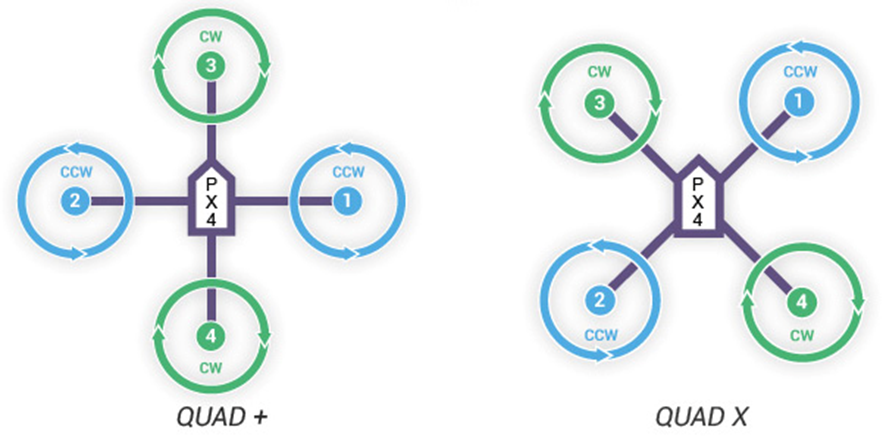
\includegraphics[width=0.65\textwidth]{Vooronderzoek/quad_configuraties.png}
					  \caption{Verschillende configuratiemogelijkheden van een quadcopter}
					  \label{quad_config}
				\end{figure}

			\par De keuze van een bepaalde configuratie heeft een invloed op de manier van besturing, maar ook op het algoritme waarmee de verschillende motoren worden aangestuurd. Wanneer men gebruikt maakt van de  \textquoteleft x\textquoteright configuratie, zijn er twee motoren nodig om een beweging om een bepaalde as uit te voeren. 

			\par Het spreekt voor zich dat het algoritme dat nodig is om de motoren aan te sturen bij een  \textquoteleft x\textquoteright configuratie complexer is dan bij de keuze van een  \textquoteleft +\textquoteright configuratie. Er wordt dus gekozen voor de  \textquoteleft +\textquoteright configuratie binnen dit projectlab.

		\subsection{Besturing van een quadcopter}
			
			\par Om een quadcopter te besturen dienen de motoren op een correcte wijze aangestuurd te worden. Afhankelijk van hoe de motoren aangestuurd worden zal de quadcopter stijgen, dalen, gieren, of stampen. Daarnaast is het ook mogelijk een combinatie van de verschillende bewegingen samen uit te voeren.

			\par Om een quadcopter te laten stijgen of dalen, dienen de vier motoren gelijktijdig versneld of vertraagd te worden. 

			\par Om een quadcopter te laten bewegen om zijn verticale as moet de snelheid van twee motoren die \'e\'enzelfde draairichting hebben verhoogd worden. Hierdoor zal het koppel op de quadcopter toenemen waardoor een gierbeweging zal ontstaan.

			\par Om een quadcopter vooruit, achteruit, link of rechts te laten bewegen in de \textquoteleft + \textquoteright  configuratie volstaat het om \'e\'en motor sneller te laten bewegen dan de anderen. Hierdoor zal de quadcopter kantelen in een bepaalde richting, met een verplaatsing tot gevolg.

			\par In figuren \ref{quad_up_down}, \ref{quad_gieren} en \ref{quad_kantelen} is een overzicht weergegeven van de besturing van een quadcopter in de \textquoteleft + \textquoteright configuratie.

		\begin{figure}[H]
			\centering
				\begin{minipage}[b]{0.3\textwidth}
					\centering
					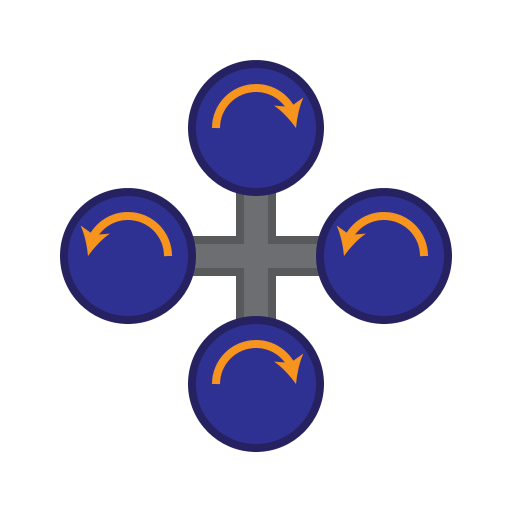
\includegraphics[height = 8cm, valign = b,width=\linewidth]{Vooronderzoek/quad_up_down.png}
					\caption[Omhoog en omlaag]{Omhoog en omlaag}
					\label{quad_up_down}
				\end{minipage}
			\quad
				\begin{minipage}[b]{0.3\textwidth}
					\centering
					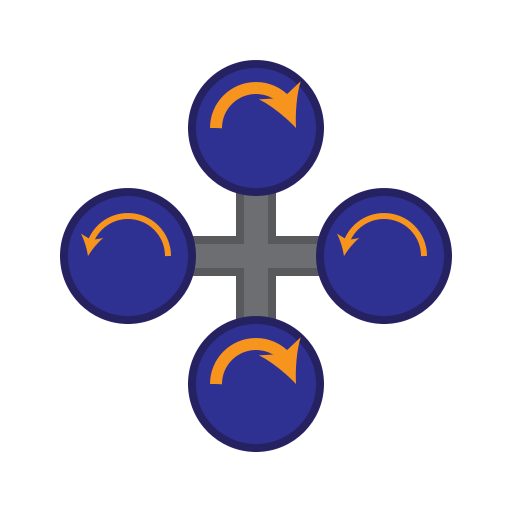
\includegraphics[height = 8cm, valign = b,width=\linewidth]{Vooronderzoek/quad_gieren.png}
					\caption[Gieren]{Gieren \newline \ }
					\label{quad_gieren}
				\end{minipage}
			\quad
				\begin{minipage}[b]{0.3\textwidth}
					\centering
					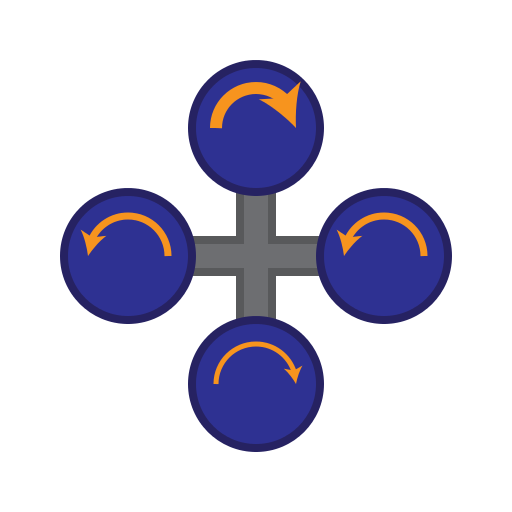
\includegraphics[height = 8cm, valign = b,width=\linewidth]{Vooronderzoek/quad_kantelen.png}
					\caption[Kantelen]{Kantelen \newline \ }
					\label{quad_kantelen}
				\end{minipage}
		\end{figure}

	\section{PID regelaar}

		\par Een PID regelaar is een veel voorkomende regelaar binnen de procesregeling. De afkorting PID staat voor Proportioneel, Integrerend en Differenti\"erend. Dit zijn ook de acties waaruit de regelaar is opgebouwd.

		\subsection{Werkingsprincipe}

			\par De regeling gaat uit van het verschil tussen de gewenste waarde en de actuele gemeten waarde. Dit wordt omschreven als het foutsignaal. Het bijsturen van dit foutsignaal gebeurt in drie parallelle stappen.

				\begin{description}
					
					\item[P-actie:] De proportionele actie zal het foutsignaal versterken met een factor K\textsubscript{p}.

					\item[I-actie:] De integrerende actie zorgt voor een constante sommatie van het foutsignaal. Afhankelijk van hoe lang er een fout is tussen de gemeten en gewenste waarde, zal de integrerende actie meer of minder signaal uitsturen. De K\textsubscript{i} term, ook wel nasteltijd genoemd, bepaald het effect van deze actie. Hoe kleiner deze waarde, hoe krachtiger de actie.

					\item[D-actie:] De differenti\"erende actie zal reageren op de snelheid van verandering van het foutsignaal. Hoe hoger de factor K\textsubscript{d} wordt ingesteld, hoe sneller de wenswaarde bereikt zal worden.

				\end{description}

			\par Wiskundig kan men een PID regelaar als volgt omschrijven:

				\[ u(t) = K_{p}\cdot (e(t)+\frac{\int e(t)dt }{T_{i}}+ T_{d}\cdot \frac{de(t))}{dt}) \]

			\par Hierin is 

				\begin{conditions*}
					U(t)				& De uitgang van de regelaar				\\
					K\textsubscript{p}	& De proportionele actie van de regelaar	\\
					T\textsubscript{i}	& De integratietijd van de regelaar			\\
					T\textsubscript{d}	& De differentiatietijd van de regelaar 	\\
					E(t)				& Het errorsignaal							\\
				\end{conditions*}

			\par Het bepalen van de juiste constanten is een werk van trial-and-error. Dit zal dan ook experimenteel moeten vastgesteld worden op de quadcopter.

		\subsection{Digitalisatie van een PID}

			\par De formule die hierboven weergegeven is, kan als volgt vertaald worden naar een digitaal systeem.

				\[ U\textsubscript{k} = U\textsubscript{k-1} \cdot e\textsubscript{k} + b\textsubscript{0} \cdot + b\textsubscript{1} \cdot e\textsubscript{(k-1)} + b\textsubscript{2} \cdot e\textsubscript{(k-2)} \]

			\par Hierbij is

				\begin{itemize}
					\item[] $ b\textsubscript{0} = K\textsubscript{p}(1+ \frac{T\textsubscript{d}}{T}) $ \\					
					\item[] $ b\textsubscript{1} = K\textsubscript{i}(-1 +  \frac{T}{T\textsubscript{i}} -2\frac{T\textsubscript{d}}{T} ) $ \\		
					\item[] $ b\textsubscript{2} = K\textsubscript{d}(\frac{T\textsubscript{d}}{T}) $ \\
				\end{itemize}

			\par Deze formule kan weergegeven worden in het onderstaande schema.
	
				\begin{figure}[H]					  
					  \centering
					  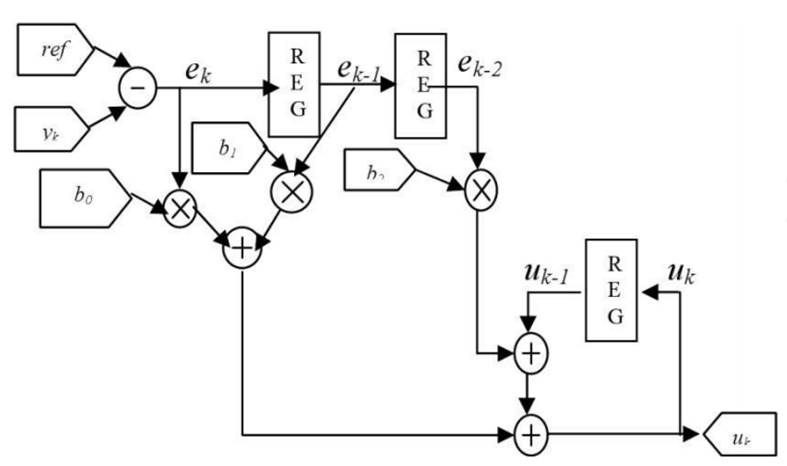
\includegraphics[width=0.8\textwidth]{Vooronderzoek/pid_digitaal_schema.png}
					  \caption{Schematische voorstelling van een PID regelaar}
					  \label{pdi_digitaal_schema}
				\end{figure}

			\par De werking van de in figuur \ref{pdi_digitaal_schema} weergegeven regelaar wordt gevalideerd via het programma Simulink. Op deze manier kan reeds voor de FPGA implementatie gekeken worden of de regelaar zal doen wat er verwacht wordt. Daarnaast vormt deze simulatie een goede basis om het FPGA design te starten. In figuur \ref{pdi_simulink_schema} is de Simulink versie van de PID regelaar weergegeven.

				\begin{figure}[H]					  
					  \centering
					  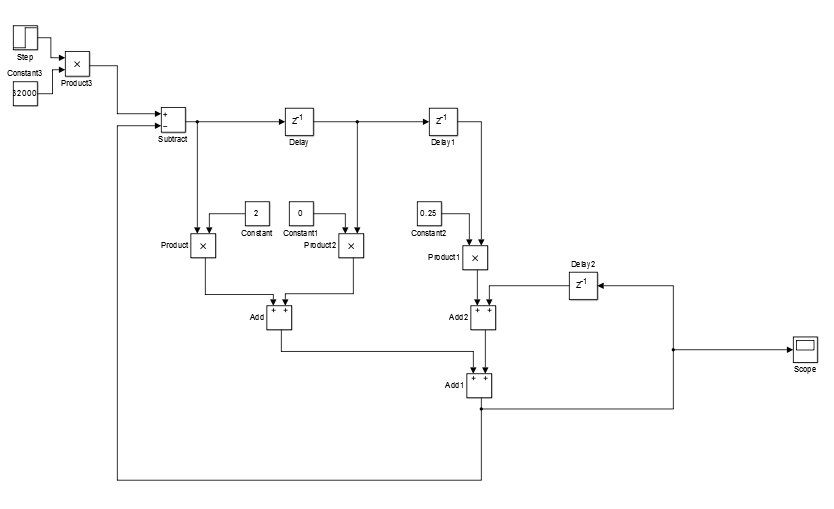
\includegraphics[width=\textwidth]{Vooronderzoek/pid_simulink_simulatie.png}
					  \caption{Simulink voorstelling van een PID regelaar}
					  \label{pdi_simulink_schema}
				\end{figure}

			\par Wanneer men de uitgang aan de ingang koppelt van bovenstaande PID wordt er aangenomen dat de nieuwe gemeten waarde gelijk is aan de uitgang van de PID. Dit levert het volgend resultaat op na simulatie.

				\begin{figure}[H]					  
					  \centering
					  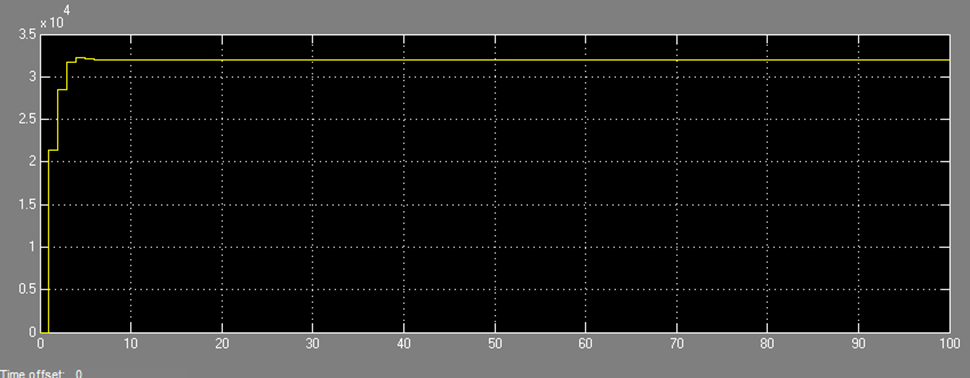
\includegraphics[width=\textwidth]{Vooronderzoek/pid_simulink_resultaat.png}
					  \caption{Resultaat van simulatie PID in Simulink }
					  \label{pdi_simulink_resultaat}
				\end{figure}

			\par In figuur \ref{pdi_simulink_resultaat} is duidelijk de werking van een PID waar te nemen. Het signaal klimt naar de gewenste waarde toe, maakt een kleine overshoot en stabiliseert vervolgens op het gewenste signaal. Dit is ook wat men verwacht van een PID. Men kan dus besluiten dat het schema in figuur \ref{pdi_digitaal_schema} voldoet aan de eisen en ge\"implementeerd kan worden in de FPGA.

	\section{Xilinx DSP48 slices}

		\par De Spartan 6 reeks bevat verschillende DSP48A slices. Deze MAC bouwstenen zijn door Xilinx speciaal ontworpen om DSP toepassingen te realiseren.

			\begin{figure}[H]					  
				  \centering
				  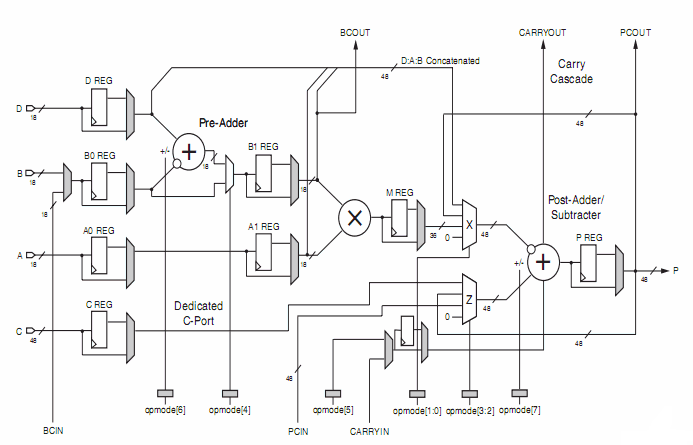
\includegraphics[width=0.90\textwidth]{Vooronderzoek/dsp48a.png}
				  \caption{Interne structuur van een DSP48A slice }
				  \label{pdi_simulink_resultaat}
			\end{figure}

		\par Het doel van een DSP48 slice is het zo performant mogelijk uitvoeren van MAC operaties. Hiervoor zijn verschillende adders en een multiplier binnen het DSP48 slice aanwezig. Als invoer kan een signaal van maximaal 18 bits aangelegd worden. De uitgang is maximaal 48 bit. Hiervan is ook de naam DSP48 afgeleid.

		\par De DSP48A slices kunnen binnen de Xilinx ISE ontwikkelomgeving op verschillende manieren worden ge\"instantieerd. De eenvoudigste methode is via de IP Coregen. De gebruiker maakt stapsgewijs de instellingen op basis van een aantal selecties. Visueel wordt weergegeven welke instellingen gemaakt worden. Een andere manier om een DSP48 Slice te implementeren is door gebruik te maken van een zogenaamde Port Map in de code. Hierbij worden alle instellingen handmatig gemaakt en dient goed rekening gehouden te worden met de datasheet. Een derde manier om DSP48 slices te gebruiken is via de Xilinx System Generator. Dit is een pakket dat in samenwerking met Matlab en Simulink de mogelijkheid voorziet om visueel, door middel van blokken, een systeem samen te stellen en de nodige VHDL code te genereren. 

		\par De Spartan 6SLX9 beschikt over 12 DSP48A slices. Binnen het FPGA zullen deze gebruikt worden waar mogelijk om het gehele proces te versnellen.
\newpage
	\section{Mojo FPGA ontwikkelbord}

		\par Tijdens het projectlab zal gebruik gemaakt worden van het Mojo FPGA ontwikkelbord. Dit bord heeft een Spartan 6 XC6SLX9 FPGA aan boord waarbij de gebruiker beschikt over 84 digitale IO pinnen. Naast de digitale IO pinnen van het Mojo bord zijn er ook 8 analoge inputs voorzien. Deze bevinden zich op een externe ATmega controller die via een SPI interface communiceert met de FPGA.

		\par Het programmeren van het Mojo bord gebeurt op eenvoudige wijze. Via het programma Mojo loader kan een \texttt{.bit} bestand naar de externe ATmega geladen. Telkens wanneer de FPGA opgestart wordt zal het laatst opgeslagen \texttt{.bit} bestand geladen worden op de FPGA. Op deze manier dient na stroomuitval niet steeds opnieuw het \texttt{.bit} bestand geladen te worden.

		\par Er zijn reeds verschillende shields op de markt die het mogelijk maken om het Mojo board verder uit te breiden. Daarnaast is het project volledig open source waardoor er zelf ook makkelijk extra hardware ontwikkeld kan worden. Alle schema\textquotesingle s en PCB layouts zijn via de website van de makers vrij verkrijgbaar.

		\par In afbeelding \ref{mojo} is het Mojo bord weergegeven. Naast de 84 digitale en 8 analoge IO pinnen beschikt het Mojo bord ook over 8 leds die verbonden zijn met de FPGA.

			\begin{figure}[H]					  
				  \centering
				  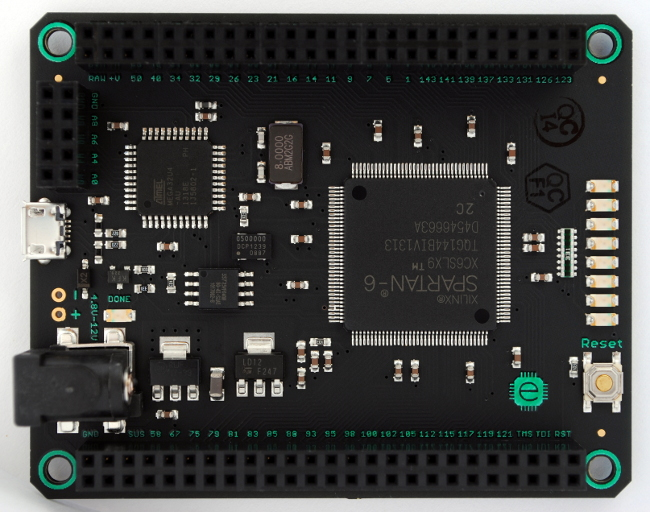
\includegraphics[width=0.6\textwidth]{Vooronderzoek/mojo.png}
				  \caption{Overzicht van het Mojo FPGA ontwikkelbord}
				  \label{mojo}
			\end{figure}
\newpage
	\section{Sensoren}

		\par Om een stabilisatie te voorzien van de quadcopter is het noodzakelijk een inzicht te krijgen van zijn actuele attitude. Hiervoor wordt gebruik gemaakt van een IMU sensor. IMU staat voor inertial measurement unit. Deze unit bevat een combinatie van accelerometers, magnetometers en gyroscopen om zo informatie te verwerven over de huidige attitude van de quadcopter in de ruimte. Om daarbij ook informatie te verschaffen over de hoogte, wordt gebruik gemaakt van de combinatie van een ultrasone sensor en een barometer.

		\subsection{Opmeten van de attitude}

			\subsubsection{Principe}

			\par Een AHRS, attitude and heading reference system, voorziet de gebruiker van informatie over de stand van het vliegtuig. Om dit te berekenen wordt gebruik gemaakt van de data die afkomstig is van een IMU sensor. Zoals reeds hierboven beschreven werd, is een IMU sensor een combinatie van volgende drie sensoren.

				\begin{description}
				
					\item[Accelerometer:] Een accelerometer meet de versnelling van de quadcopter, vaak uitgedrukt in g-krachten. Aan de hand van deze versnelling kan bepaald worden of de quadcopter in een bepaalde richting beweegt of in vrije val is.
				
					\item[Gyroscoop:] Een gyroscoop meet de hoekverdraaiing op, uitgedrukt in radialen per seconde. Zo kan men de draairichting van de quadcopter bepalen. Deze hoekverdraaiing kan op zijn beurt gebruikt worden om de gemeten accelerometerwaarden te corrigeren. Indien de accelerometer namelijk niet in de correcte positie gehouden wordt, is het assenstelsel van de quadcopter verdraaid en zijn de gemeten x, y en z componenten niet correct ten opzichte van het assenstelsel in de re\"ele wereld.

					\item[Magnetometer:] Een magnetometer meet storingen in het aardmagnetisch veld op. Deze data wordt gebruikt om de performatie van de AHRS berekeningen op te voeren.
				
				\end{description}

			\par Aangezien men met de gyroscoop kan opmeten hoe groot de verdraaiing ten opzichte van het originele assenstelsel is, kunnen we het assenstelsel van de accelerometer corrigeren door matrixbewerkingen uit te voeren. Op die manier zijn de gemeten accelerometerwaarden toch te beschouwen vanuit het wereldse assenstelsel.

			\par Uit deze data wordt vervolgens de attitude van de quadcopter berekend. Deze bestaat uit de heading, de pitch-rate en de yaw-rate. 

			\par Vele sensoren gebruiken naast de boven beschreven parameters ook de temperatuur om een kalibratie uit te voeren en de nauwkeurigheid van het systeem te verbeteren.

			\par In figuur \ref{ahrs} is het principe van een AHRS op basis van IMU data weergegeven. 
			
			\begin{figure}[H]					  
				  \centering
				  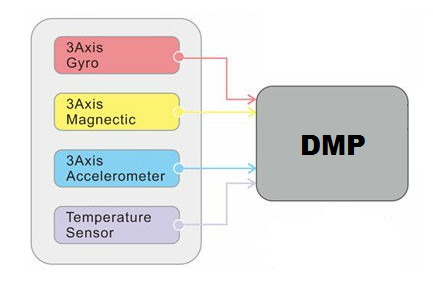
\includegraphics[width=0.6\textwidth]{Vooronderzoek/ahrs.png}
				  \caption{Overzicht van een AHRS systeem}
				  \label{ahrs}
			\end{figure}


			\subsubsection{Sensoren}

				\par Vandaag de dag zijn er verschillende sensoren op de markt te verkrijgen. Onderzoek heeft uitgewezen dat binnen de UAV wereld de MPU reeks van InvenSense vaak gebruikt worden als IMU. Binnen deze reeks van sensoren komen twee sensoren in aanmerking.

					\begin{description}

						\item[MPU 6050:] Deze IMU omvat heel wat mogelijkheden. Zo is er een ingebouwde processor, de DMP (Digital Motion Processor), die reeds heel wat berekeningen op zich kan nemen. Deze DMP is in staat simpele gestures te detecteren, stappen te tellen, filtering uit te voeren van de sensorwaarden en meer aangezien deze volledig naar wens kan ingesteld worden. De nauwkeurigheid van deze IMU is uitstekend, alsook de mogelijkheid tot het herconfigureren van de DMP. De MPU 6050 bevat een 3-assige accelerometer en een 3-assige gyroscoop. Via een I\textsuperscript{2}C is het mogelijk een externe magnetometer aan te sluiten. De data hiervan wordt opgenomen in de DMP bewerkingen.
						
						\item[MPU 9250:] Deze IMU beschikt over exact dezelfde mogelijkheden als de MPU 6050, maar heeft reeds een 3-assige magnetometer aan boord. Er dient dus geen externe magnetometer aangesloten te worden.

					\end{description}

				\par Er werd gekozen om de MPU9250 sensor te gebruiken bij het ontwerp van de quadcopter. Door de interne filter binnen de DMP wordt een Kalman filter overbodig in het FPGA ontwerp.

		\section{Serial peripheral interface}

			\par SPI is een veelgebruikt protocol voor communicatie tussen twee apparaten. Een SPI-bus bestaat uit vier signalen.

				\begin{description}

					\item[MOSI:] (Master Out Slave In) Dit signaal is de uitgang van de master en vormt de ingang van het slave apparaat. Via dit kanaal wordt informatie van de master naar de slave verstuurd.

					\item[MISO:] (Master In Slave Out) Dit signaal is de uitgang van de slave en vormt de ingang van het master apparaat. Via dit kanaal wordt informatie van de slave naar de master verstuurd.

					\item[SCLK:] (Serial Clock Line) Dit kanaal wordt gebruikt als klok. Het is het master apparaat dat de klok voorziet voor het slave apparaat. Data wordt enkel verstuurd en ontvangen als er een kloksignaal is.

					\item[SS:] (Slave Select) Via een slave select kan de master kiezen uit verschillende slave apparaten waarmee hij wil communiceren. Op deze manier kan een communicatie opgezet worden met meerdere apparaten door middel van \'e\'en master apparaat.

				\end{description}

			\par Zoals reeds eerder werd aangehaald, bestaat een SPI interface uit \'e\'en master apparaat en verschillende slave apparaten. Hierbij kan de master communiceren met elke slave, maar een slave kan enkel communiceren met de master. Aan de hand van een uniek slave select signaal voor elke slave wordt de selectie gemaakt. De communicatie gebeurt full duplex. 

			\par De vereiste voor de klok is dat zijn frequentie lager moet zijn dan de maximale frequentie van de betrokken toestellen. Binnen SPI zijn er twee parameters waarbij rekening gehouden moet worden.


				\begin{description}

					\item[CPOL:] De Clock polarity geeft aan wat de standaard waarde is van het kloksignaal wanneer de SPI-bus zich in de idle toestand bevindt. 

					\item[CPHA:] De Clock phase geeft aan op welke edge van het signaal gesampled zal worden. Een 0 geeft aan dat er op de rising edge gesampled wordt. Een 1 geeft aan dat er op de falling edge gesampled wordt.

				\end{description}

			\par Door het combineren van bovenstaande parameters kan men vier verschillende modi onderscheiden binnen de SPI interface. In figuur \ref{spi_clock} is een overzicht weergegeven van een SPI communicatie tussen twee apparaten. Hierbij zijn de CPOL en CPHA beide ingesteld op 0.

				\begin{figure}[H]					  
					  \centering
					  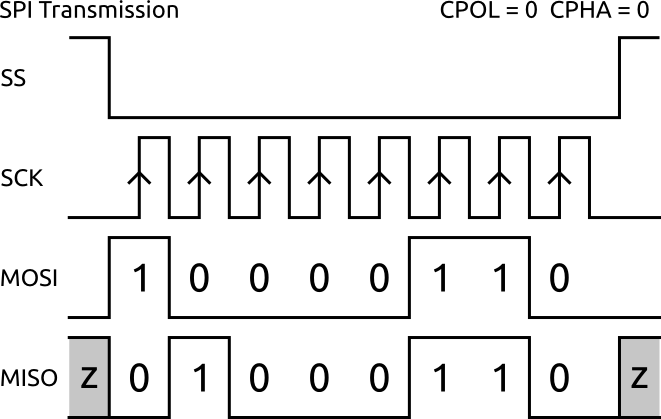
\includegraphics[width=0.6\textwidth]{Vooronderzoek/spi.png}
					  \caption{Overzicht van SPI communicatie tussen master en slave}
					  \label{spi_clock}
				\end{figure}

			\par Op het moment dat de master een clock genereert, zal de communicatie aanvatten. Zowel de master als de slave zullen gelijktijdig data uitwisselen.  

			\par Wanneer de SS naar een lage toestand gebracht wordt, zal de slave geselecteerd worden. Vervolgens genereert de master het kloksignaal en start daarbij ook met versturen van data. Het slave apparaat zal ook starten met sturen van data op de wijzigende flanken van de klok. Wanneer de communciatie voltooid is, stopt de klok en wordt de SS weer naar hoge toestand gebracht.

			\par Om data van de slave op te vragen, moet dus eerst een bericht verzonden worden van welke data men wil opvragen. Daarna moet men nog een bericht versturen om de data te ontvangen. Dit is nodig aangezien het zenden en ontvangen steeds gelijktijdig gebeurt.
\newpage
		\section{Systeemoverzicht}

			\par De resultaten van dit vooronderzoek hebben geleid tot een systeem dat in staat is om de attitude van de quadcopter te controleren. Dit systeem dient in de volgende fase van het project ge\"implementeerd te worden in een FPGA. In figuur \ref{systeemoverzicht} is een overzicht van dit systeem weergegeven.

				\begin{figure}[H]					  
					  \centering
					  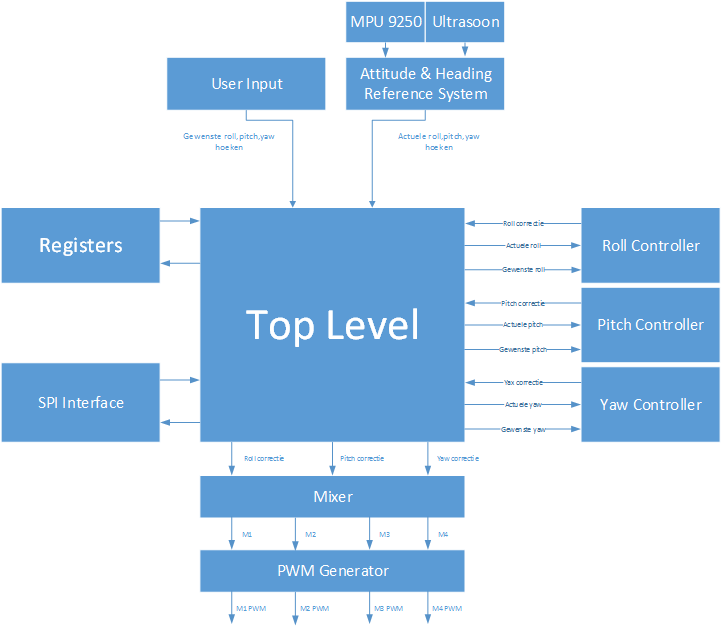
\includegraphics[width=\textwidth]{Vooronderzoek/blokschema.png}
					  \caption{Schematische voorstelling van de quadcopter autopilot}
					  \label{systeemoverzicht}
				\end{figure}
\newpage
			\par In de figuur kan men volgende blokken onderscheiden.

				\begin{description}

					\item[User input:] Deze blok is verantwoordelijk voor het afhandelen van de gebruikersinvoer. Deze is afkomstig van de RF antenne. Een PWM signaal per kanaal dient gelezen te worden. Dit PWM signaal wordt door het toplevel doorgegeven aan de PID controllers om zo de gewenste actie te ondernemen.

					\item[Registers:] In de registers worden alle verschillende instellingen bewaard. Naast deze instellingen worden ook waarden aangeboden aan de gebruiker. Via een SPI interface kan het register gelezen en beschreven worden.

					\item[SPI interface:] De SPI slave interface maakt het mogelijk om zowel te communiceren met een externe microcontroller als de MPU9250 die dienst doet als IMU uit te lezen.

					\item[Mixer:] De mixer is verantwoordelijk voor de verwerking van alle data die afkomstig is van de PID controllers voor rol, pitch en yaw. Aan de hand van deze informatie zal de mixer de geschikte PWM waarden berekenen voor de motoren. Hierbij zal rekening gehouden worden met de maxima en minima die ingesteld zijn in de registers.

					\item[PWM generator:]  De BLDC motoren worden aangestuurd door middel van een PWM signaal. De PWM generator zal voor elke motor een geschikt PWM signaal genereren op basis van de uitvoer van de mixer.

					\item[Roll controller:] De roll-controller stabiliseert het rollkanaal van de quadcopter. Naast de gebruikersinvoer vormt ook de roll-info van het AHRS een input voor deze controller.

					\item[Pitch controller:] De pitch-controller stabiliseert het pitchkanaal van de quadcopter. Naast de gebruikersinvoer vormt ook de pitch-info van het AHRS een input voor deze controller.

					\item[Yaw controller:]De yaw-controller stabiliseert het yawkanaal van de quadcopter. Naast de gebruikersinvoer vormt ook de yaw-info van het AHRS een input voor deze controller.

					\item[Attitude \& heading reference system:] Het AHRS geeft meer informatie over de attitude en heading van de quadcopter. Hiervoor gebruikt dit systeem verschillende sensoren. Dit AHRS systeem zal uitgevoerd worden op een aparte microcontroller en via een SPI interface waarden doorgeven aan het autopilot systeem.

				\end{description}

			\par In het volgende hoofdstuk zullen alle stappen besproken worden die nodig zijn om bovenstaande blokken te implementeren.
\chapter{Implementatie}

	\par In dit hoofdstuk zal de implementatie van het volledige systeem besproken worden. Er zal vooral de nadruk gelegd worden op de moeilijkheden en problemen die zich voordeden tijdens het ontwikkelproces.

	\section{PID regelaar}

		\par De PID regelaar vormt het belangrijkste onderdeel van de quadcoptersturing. Deze component zal per as ge\"implementeerd moeten worden. Daarnaast kan de PID in een verder stadia ook gebruikt worden om de hoogte te stabiliseren. Er dient dus een flexibele component ontworpen te worden die meerdere malen ingezet kan worden. Hierbij is het belangrijk dat de waarden voor K\textsubscript{p}, K\textsubscript{i} en K\textsubscript{d} per controller ingesteld kunnen worden. Daarnaast is het ook mooi meegenomen om deze real-time aanpasbaar te maken. 

		\par De PID controller werd ontwikkeld in drie iteraties. Vanwege de hardware beperkingen van de FPGA was het nodig om een volledig re-design uit te voeren van de component. Deze stappen zullen hieronder verder toegelicht worden.

		\subsection{PID controller door middel van DSP48A slices}

			\par Vanuit theoretisch oogpunt zijn DSP48 slices ideaal voor het implementeren van een PID regelaar. De bewerkingen die uitgevoerd dienen te worden beperken zich tot optellen en vermenigvuldigen (MAC). Op deze manier wordt een hoge snelheid van de component mogelijk. Per PID regelaar zijn vier DSP48 slices nodig. In figuur \ref{pid_dsp48} is de onderverdeling weergegeven van DSP48 slices binnen de PID regelaar. Hierbij zijn de functies van slice 2 en 3 exact hetzelfde. Bij de laatste DSP48 slice is een terugkoppeling voorzien. Om ervoor te zorgen dat het resultaat nooit overflowt, dient er een downscaling te gebeuren bij de terugkoppeling. Deze wordt in \textquotesingle gewone\textquotesingle   logica uitgevoerd en zal het proces vertragen. Door het introduceren van de nodige \textquotesingle pipes\textquotesingle  wordt de maximale snelheid van implementatie bereikt.
				
				\begin{figure}[H]					  
					  \centering
					  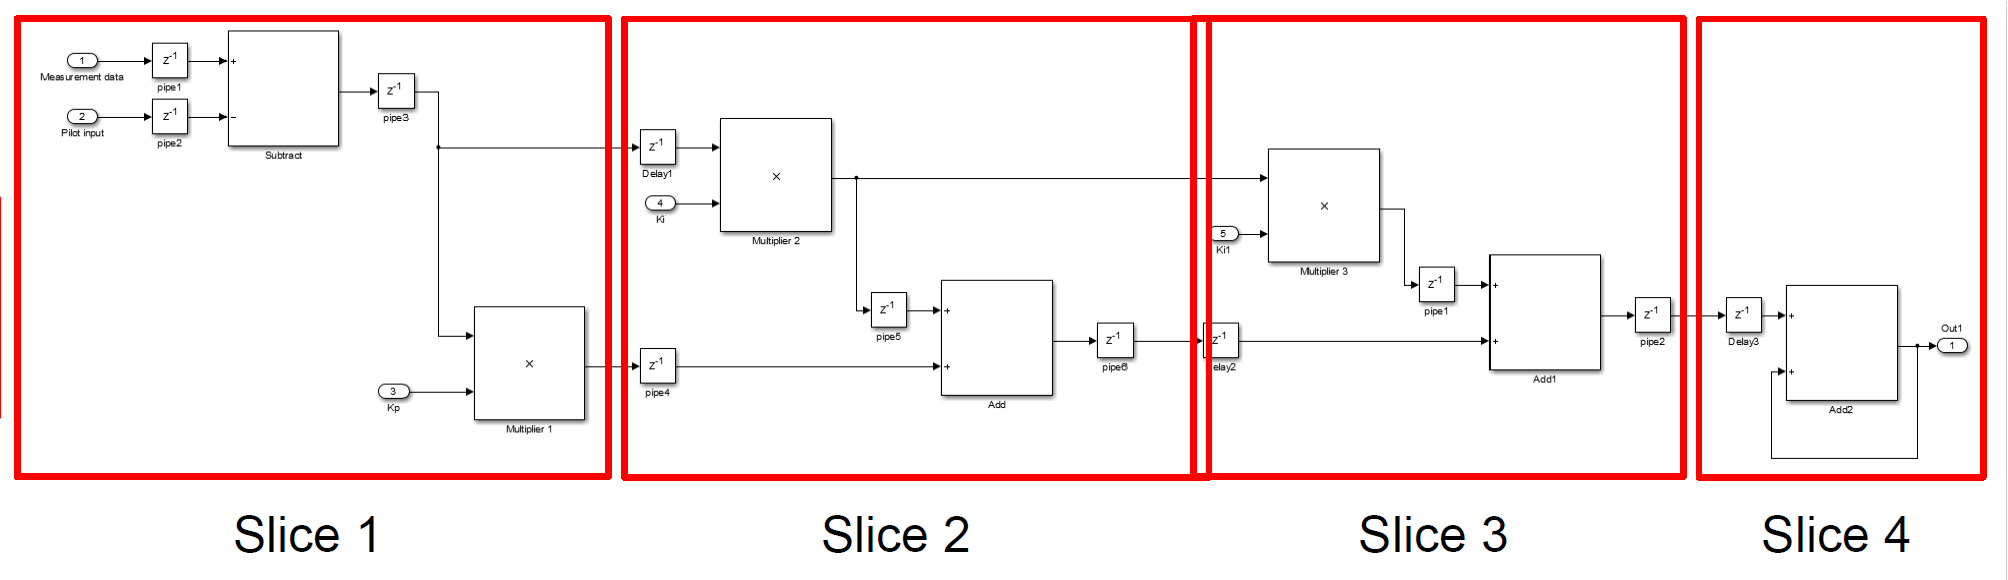
\includegraphics[width=\textwidth]{Implementatie/pid_dsp48.png}
					  \caption{Overzicht van een PID controller op basis van DSP48 slices}
					  \label{pid_dsp48}
				\end{figure}

			\par Bovenstaande code werd in een eerste fase ge\"implementeerd door middel van de Xilinx System Generator. Wanneer de VHDL code gegenereerd diende te worden, doken er steeds fouten op. Opzoekwerk heeft uitgewezen dat de System Generator niet compatibel is met Windows 8. Een Windows 7 apparaat met alle nodige software en licenties was helaas niet beschikbaar. Er werd overgegaan naar het implementeren van de PID in Xilinx ISE. Hierbij werd gebruik gemaakt van de IP Coregen voor het genereren van de juiste instellingen binnen de DSP48 slices.

			\par Door eerste synthese resultaten bleek dat het niet mogelijk was om drie of vier PID's te implementeren op de Spartan 6 FPGA wegens gebrek aan resources. Een mogelijke oplossing was het multiplexen van de PID regeling. Op die manier is er slechts \'e\'en PID regelaar nodig die afwisselend de berekeningen uitvoert voor een bepaald kanaal. De implementatie hiervan bleek echter te complex om te realiseren omdat de PID steeds de vorige resultaten nodig heeft om het volgende te berekenen. Deze data zou dus moeten opgeslagen worden. Daarnaast was het ook niet steeds mogelijk om deze waarden terug op de juiste plaats in het DSP48 slice te laden vanwege de beperkingen van ingangssignalen.

			\par Er dient dus een andere oplossing gevonden te worden om de PID in de Spartan 6 FPGA te implementeren.

		\subsection{PID controller door middel van IPCore multiplier}
		\label{pid_mult}

			\par Een tweede aanpak was om de PID te implementeren aan de hand van \textquotesingle gewone\textquotesingle  logica. Om de vermenigvuldigingen uit te voeren wordt gebruik gemaakt van de IP Core multiplier. Er zijn dus drie van deze multipliers nodig om de volledige component te realiseren. 

			\par Bij het aanmaken van deze multipliers zijn verschillende keuzes mogelijk. Er kan gekozen worden tussen een implementatie die gebruik maakt van ExtremeDSP (DSP48A slices) of een implementatie die gebruik maakt van LUT's en FF. Afhankelijk van de gekozen optie zullen de timings verschillen. Er is ook een mogelijk om te optimaliseren naar area (minimaal gebruik aan resources) of naar snelheid. Er werd gekozen om te minimaliseren naar area. Hierbij maakte de multiplier enkel gebruik van LUT's en FF. 

			\par Via Xilinx Vivado werd een eerste versie van deze PID ge\"implementeerd en gesimuleerd. De keuze voor Vivado werd gemaakt omwille van problemen met de ISE simulator op Windows 8. Daarnaast was het ook niet mogelijk om CoreIP componenten te simuleren in Modelsim vanwege een probleem met de bibliotheken. Xilinx biedt deze niet meer aan, omdat zij een eigen simulator ontwikkeld hebben.

			\par De simulaties leverden dezelfde resultaten op als bekomen in Simulink. Er kon dus besloten worden dat de implementatie van de PID gelijkaardig is als de versie in Simulink. Bij het verder onderzoeken van de synthese resultaten bleek dat er op het eerste zicht voldoende resources beschikbaar waren om vier PID controllers te implementeren. Omdat er niet enkel een PID op de FPGA ge\"implementeerd moet worden, maar ook nog een reeks andere componenten zou het toch kunnen dat men niet voldoende resources ter beschikking heeft.

			\par  Er dient dus een andere oplossing gevonden te worden om de PID in de Spartan 6 FPGA te implementeren met een minimaal gebruik aan resources.

		\subsection{PID controller door middel van multiplexed IPCore multiplier}			

			\par Een oplossing om de resources binnen een PID controller aanzienlijk te beperken is door in plaats van drie multipliers slechts \'e\'en multiplier te gebruiken. Hierbij zal telkens de P, I en D actie uitgevoerd worden. De snelheid van het component zal hierdoor dalen met ongeveer een facor drie, maar dit zal weinig invloed hebben op de werking van de autopilot. Aangezien de sensordata binnenkomt met een snelheid van enkele kHz en de PID component geklokt kan worden aan een snelheid van enkele MHz zal hier geen effect van opgemerkt kunnen worden.

			\par De implementatie gebeurt door middel van een state machine. In een eerste state zullen de  K\textsubscript{p}, K\textsubscript{i} en K\textsubscript{d} waarden ingelezen worden. Op deze manier zijn ze per berekening real-time aanpasbaar. In de volgende states zullen de P, I en D acties uitgevoerd worden. Dit houdt in dat de data die aan de multiplier aangelegd wordt, wijzigt per state. In de laatste state wordt een vlag kort hoog geplaatst om aan te geven dat de berekening klaar is. Er is dus maar \'e\'en multiplier nodig die gemultiplext wordt.

			\par Door het beperken van het aantal multipliers kon de snelheid van de multiplier geoptimaliseerd worden door toch gebruik te maken van DSP48 slices binnen deze multiplier. Deze wijziging werd dan ook doorgevoerd in de component.
\newpage
			\par Simulaties van de bovenstaande PID leverden exact hetzelfde resultaat op als de PID beschreven in paragraaf \ref{pid_mult}. Een overzicht van deze testbench is weergegeven in figuur \ref{pid_tb_mult}.

				\begin{figure}[H]					  
					  \centering
					  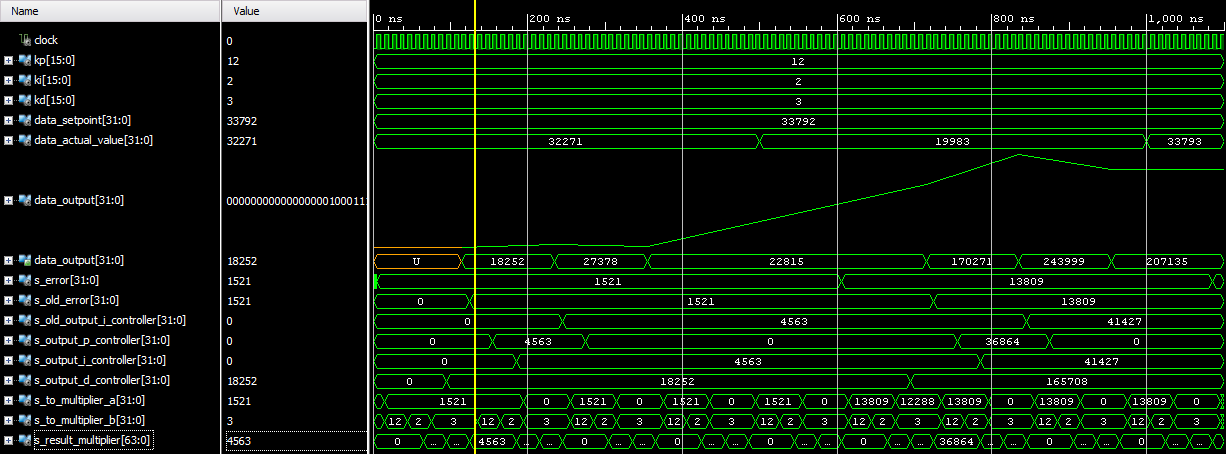
\includegraphics[width=\textwidth]{Implementatie/pid testbench.png}
					  \caption{Simulatieresultaat van PID regelaar met gemultiplext multiplier}
					  \label{pid_tb_mult}
				\end{figure}

			\par Wanneer men figuur \ref{pid_tb_mult} nader bekijkt, kan men opmerken dat wanneer de wenswaarde bereikt is, en bijgevolg het errorsignaal 0 is, de uitvoer niet terugvalt naar 0. De reden hiervoor is eenvoudig te verklaren. Aangezien de testbench werkt door middel van het aanleggen van bepaalde signalen voor gemeten waarde op bepaalde tijdstippen, heeft men hier niet te maken met een echt systeem. De I actie van de PID wordt berekend door middel van volgende formule.

				\[ I\textsubscript{regelaar} = (Error \cdot K\textsubscript{i} + Old_K\textsubscript{i} ) \] 

			\par Er wordt dus steeds een berekening gemaakt op basis van de oude waarde van K\textsubscript{i} waardoor de waarde nooit 0 wordt in de simulatie. In een echt systeem wordt dit probleem onmiddellijk opgelost omdat de regelaar zal blijven bijregelen. De sensor zal opmerken dat de waarde de wens overstijgt en een tegenactie ondernemen. 


		\subsection{Samenvattig PID controller}

			\par In listing \ref{PID_list_1} is de componentdefinitie van de PID controller weergegeven. Als invoer zijn zowel de sensordata als de gewenste waarde nodig. Daarnaast moeten ook de co\"effici\"enten voor  K\textsubscript{p}, K\textsubscript{i} en K\textsubscript{d} aangelegd worden. Deze co\"effici\"enten zijn real-time aanpasbaar.
\newpage
			\par Door de PID regelaar in verschillende stappen te ontwerpen konden steeds resources bespaard worden. Dit ging wel steeds ten koste van de snelheid van de component. Hoge snelheid bij deze component is niet zo belangrijk vanwege de relatief trage snelheid weermee de invoerdata kan aangeleverd worden. 

				\lstinputlisting[style=vhdl, caption=Overzicht van de PID component, label=PID_list_1]{Implementatie/pid.vhd}

	\section{PWM generator}

		\par Per motor is er telkens \'e\'en PWM generator nodig bij de quadcopter. De PWM generator zal een PWM signaal genereren op basis van een invoerwaarde die afkomstig is van de motormixing component. Om flexibiliteit te garanderen is de component volledig generiek gemaakt. Op deze manier kan zowel de resolutie als PWM frequentie gewijzigd worden. Een overzicht van de PWM component is weergegeven in listing \ref{pwm_gen}. 

			\lstinputlisting[style=vhdl, caption=Overzicht van de PWM component, label=pwm_gen]{Implementatie/pwm_gen.vhd}

	\section{Motor Mixing}

		\par Het motormixing gedeelte van de quadcopter is verantwoordelijk voor het genereren van de signalen die naar elke motor gestuurd moeten worden. Bij de opbouw van de quadcopter werd gekozen voor de \textquotesingle +\textquotesingle  configuraties. Het mixen van de motors gebeurt dan via het volgend algoritme.

			\[ Motor\textsubscript{front} = baseSnelheid + pitchOutput - yawOutput \]
			\[ Motor\textsubscript{left} = baseSnelheid + rollOutput + yawOutput \]
			\[ Motor\textsubscript{back} = baseSnelheid - pitchOutput - yawOutput \]
			\[ Motor\textsubscript{right} = baseSnelheid - rollOutput + yawOutput \]

		\par Hierbij is de baseSnelheid gelijk aan de idle snelheid van de motor vermeerderd met de throttle.

		\par Net als bij de PWM generator is ook deze component volledig generiek opgebouwd zodat deze makkelijk kan aangepast worden. Een overzicht van deze component is weergegeven in listing \ref{motormixing}.

			\lstinputlisting[style=vhdl, caption=Overzicht van de motormixing component, label=motormixing]{Implementatie/motormixing.vhd}

		\par Er zal ook rekening gehouden worden met de maxima waarde van het systeem. Wanneer een bepaalde waarde het maximum overschrijdt zal deze waarde automatisch worden teruggebracht naar de maximum waarde. De corrigerende actie zal daarom wat minder zijn dan gevraagd, maar de quadcopter blijft op deze manier wel binnen zijn limieten.

	\section{SPI slave interface}

		\par Zoals reeds eerder vermeld werd, voorziet de SPI interface de mogelijkheid om de autopilot te laten communiceren met de buitenwereld. In het vooronderzoek werd reeds de werking van een SPI slave interface aangehaald. Deze is in VHDL ge\"implementeerd voor CPOL en CPHA waarbij beiden gelijk zijn aan 0. Als databreedte werd gekozen voor 8 bits, ofwel 1 byte.

		%\par Via de SPI slave interface is het ook mogelijk om toegang te krijgen tot de analoge pinnen van het Mojo board. Dit kan in het verdere verloop van het project nodig zijn. 

		\par In  listing \ref{spi_slave} is een overzicht weergegeven van het SPI slave component. Er kan data ingevoerd worden die verstuurd moet worden. Daarnaast wordt er ook kort een vlag hoog geplaatst wanneer de data ontvangen is.

			\lstinputlisting[style=vhdl, caption=Overzicht van de SPI slave component, label=spi_slave]{Implementatie/spi_slave.vhd}

		\par Om de werking van deze component te valideren, is er een testbench voor deze component ontworpen. Deze wordt geanalyseerd alvorens de code te testen op het Mojo board. Het resultaat van deze testbench is weergegeven in figuur \ref{spi_slave_tb}.

				\begin{figure}[H]					  
					  \centering
					  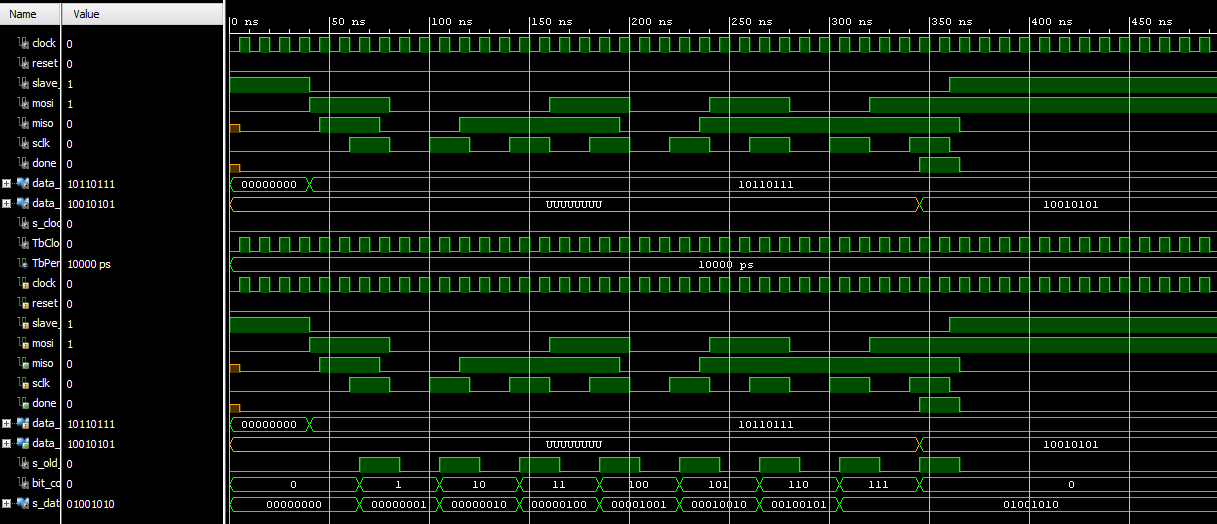
\includegraphics[width=0.9\textwidth]{Implementatie/spi_tb.png}
					  \caption{Simulatieresultaat van SPI slave interface}
					  \label{spi_slave_tb}
				\end{figure}

	\section{Top level}

		\par Het toplevel verbindt alle systeemcomponenten met elkaar. Daarnaast is ook op dit niveau de register ge\"implementeerd aan de hand van de IP Coregen. Er wordt gebruik gemaakt van een block memory met 255 registers die elk een grootte hebben van 1 byte. Via de SPI interface kunnen deze registers zowel gelezen als ingesteld worden.

		\par Het toplevel zal ook de nodige signalen naar de buitenwereld brengen. Zo worden de signalen naar de motoren, SPI-apparaten en sensoren naar buiten gebracht. 

		\par Via de IP Core clocking wizard worden de verschillende klokken aangemaakt waarmee de componenten werken. 

	\section{Quadcopter Frame}

		\par Niet alleen de hardware componenten werden ontwikkeld tijdens dit projectlab, ook de quadcopter zelf werd ontworpen. Hierbij wordt gebruik gemaakt van een 3D printer die de verschillende onderdelen zal vervaardigen. In het computerprogramma Inventor worden alle onderdelen getekend en klaargemaakt om te kunnen worden geprint.

		\par Een quadcopter is opgebouwd uit vier armen die gepositioneerd zijn in een \textquotesingle x\textquotesingle. Zo\textquotesingle n arm is weergegeven in figuur \ref{quad_frame_pict}. 

			\begin{figure}[H]					  
				  \centering
				  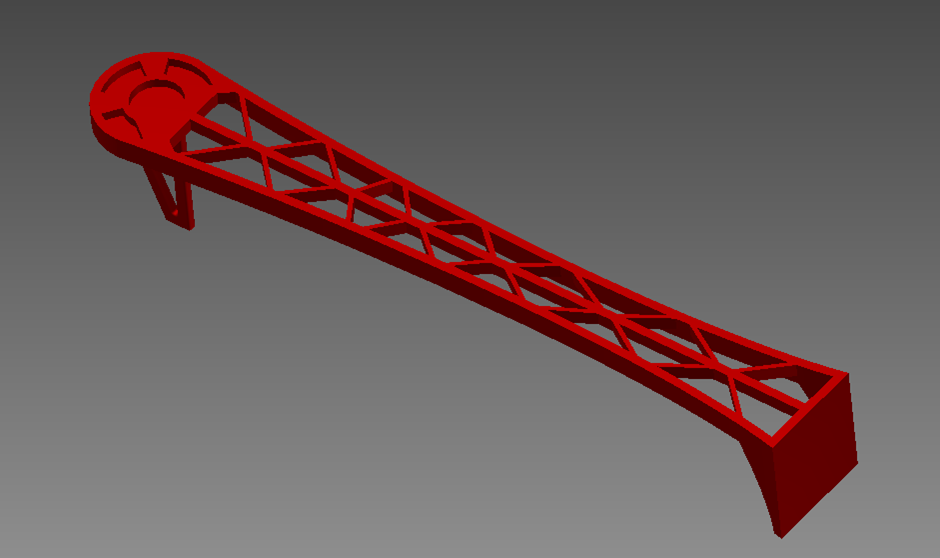
\includegraphics[width=0.6\textwidth]{Implementatie/frame.png}
				  \caption{Weergave van een quadcopter arm}
				  \label{quad_frame_pict}
			\end{figure}

		\par De frameonderdelen werden vervaardigd door middel van een Ultimaker 3D printer. Indien er tijdens de vlucht een bepaald onderdeel beschadigd raakt, kan dit makkelijk opnieuw geprint worden en is quadcopter snel weer operatief. Het printen van een arm neemt ongeveer 4 uur in beslag.






%\include{Chapter_3/hfdst-3}
%\include{Chapter_4/hfdst-4}
%\include{Chapter_5/vooronderzoek}
\include{Besluit/besluit}


% Indien er bijlagen zijn:
\appendixpage*          % indien gewenst
\appendix
\chapter{Bijlage 1 - Projectplanning}
\label{app:A}


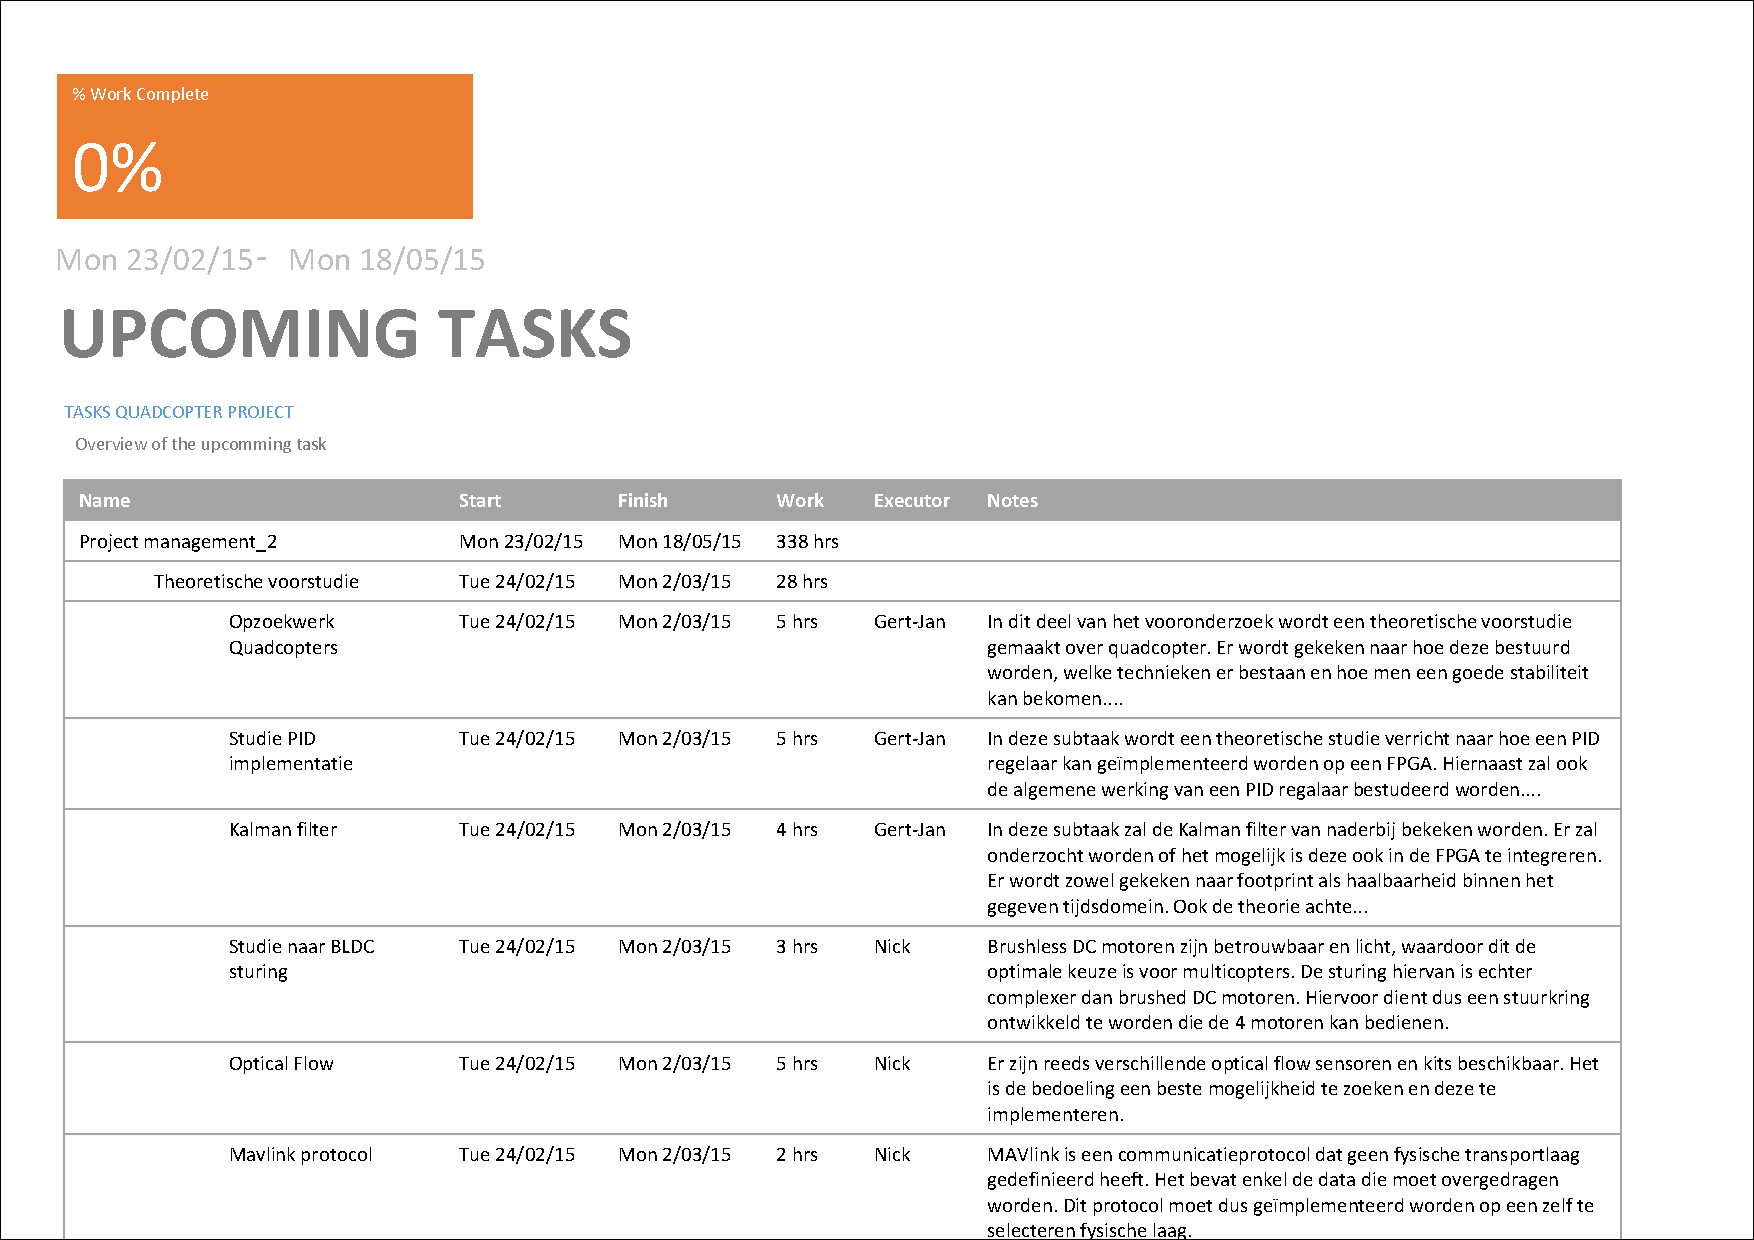
\includepdf[pages={1}, landscape= true]{Appendix/project.pdf}
\includepdf[pages={2}, landscape= true]{Appendix/project.pdf}
\includepdf[pages={3}, landscape= true]{Appendix/project.pdf}
\includepdf[pages={4}, landscape= true]{Appendix/project.pdf}
% ... en zo verder tot
%\include{Appendix/app-n}

\backmatter
% Na de bijlagen plaatst men nog de bibliografie.
% Je kan de  standaard "abbrv" bibliografiestijl vervangen door een andere.
%\bibliographystyle{abbrv}
%\bibliography{referenties}

\end{document}

